\documentclass[11pt,letterpaper,notitlepage]{article}

% Codificación GNU/Linux
\usepackage[utf8]{inputenc}
\usepackage[activeacute,spanish]{babel}

% Margenes
\usepackage{anysize}
\marginsize{2cm}{2cm}{2cm}{2cm}

% Simbolos y letras para matemáticas
\usepackage{amssymb,amsmath,amsfonts}

% Colores
\usepackage{color}
\definecolor{rojo}{RGB}{255,26,34}
\definecolor{gris}{RGB}{104,108,113}

% Elementos Flotantes (Figuras y Tablas)
\usepackage{graphicx}
\graphicspath{ {img/} }
\usepackage{float}
\usepackage{multicol}
\usepackage{multirow}
\usepackage{subfigure}
\usepackage{epstopdf}
\usepackage{enumerate}
\usepackage{hyperref}
\hypersetup{
    colorlinks,
    linkcolor={gris},
    citecolor={gris},
    urlcolor={gris}
}
\usepackage{color}
\definecolor{gray}{rgb}{0.8,0.8,0.8}
\usepackage{listings}
\lstset{ %
  backgroundcolor=\color{gray},  % keyword style
  language=c++                 % the language of the code
}
\usepackage{siunitx}

\begin{document}

% Cabezera
\begin{figure}
\vspace*{-1cm}
\begin{minipage}[c]{0.4\textwidth}
	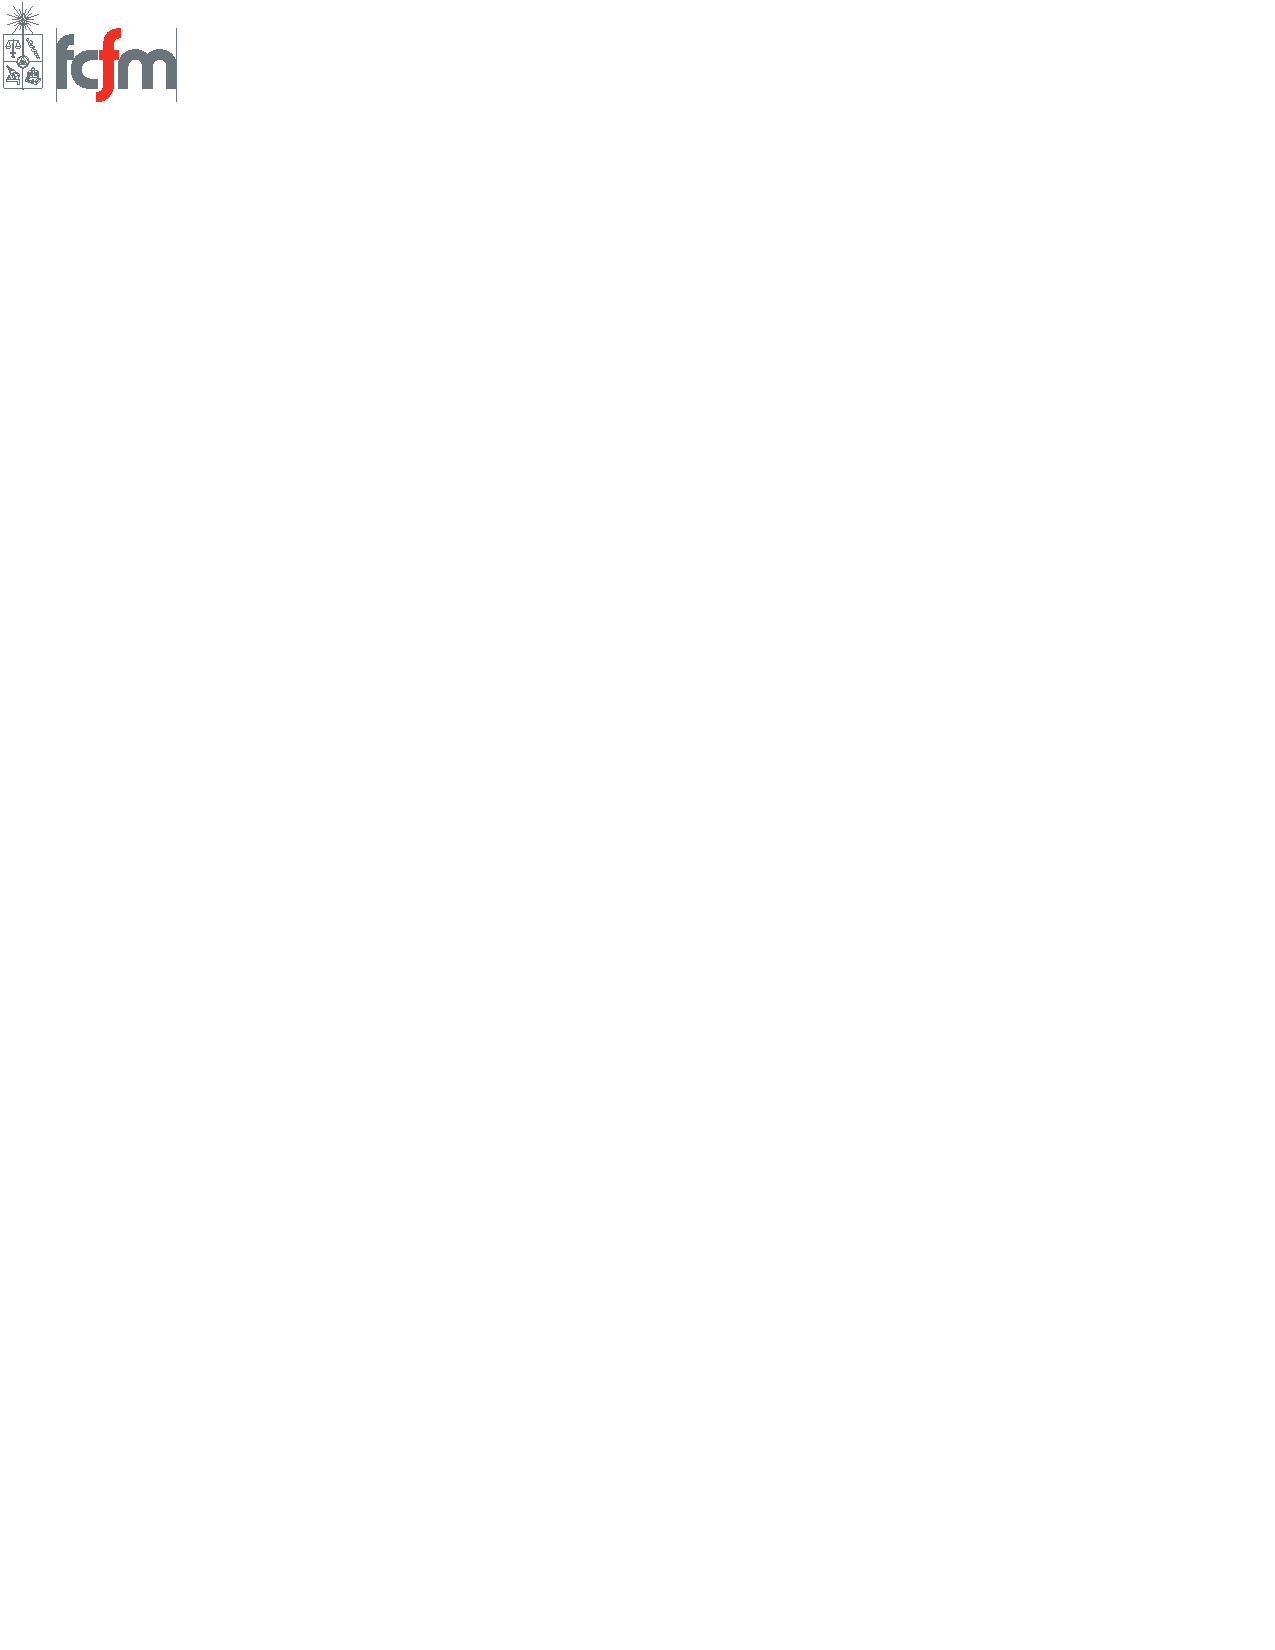
\includegraphics[width=0.5\textwidth]{fcfm}
\end{minipage}
\hfill
    \begin{minipage}[t]{0.6\textwidth}
    %--------- Datos del curso ------------------
    \begin{flushright}
    	Laboratorio de Automática\\
    	Primavera 2016 \\
    \end{flushright}
\end{minipage}
\rule{\linewidth}{.4mm}
\end{figure}

%--------- Datos del documento -------------
\begin{center}
\huge \textbf{Control de nivel para estanque cuadrado} \\
\Large \textbf{Tema: Modelamiento y control clásico}\\
\large Profesor: Roberto Cárdenas\\
\large Profesor Auxiliar: Mauricio Espinoza\\
\large Ayudantes: Ignacio Barriga, María Fernanda Fica, Rodrigo Muñoz\\
\end{center}

\section{Introducción}

En esta experiencia de laboratorio tiene como objetivo diseñar e implementar controladores PI, comparar resultados teóricos, obtenidos mediante simulaciones, con resultados experimentales de una planta real.

\subsection{Control de nivel para estanques de almacenamiento de agua}

Los controles de nivel máximo del agua en un estanque de almacenamiento tienen la función de garantizar la seguridad de las estructuras y de evitar el desperdicio de agua. El control de nivel máximo se hace mediante un sensor de nivel conectado, ya sea mecánica o electrónicamente, con la operación de una válvula a la entrada del estanque. El control de nivel mínimo del agua tiene la función de garantizar el buen funcionamiento del sistema evitando la entrada de aire en la tubería que se encuentra aguas abajo del estanque. En este caso, el sistema está compuesto por un sensor de nivel conectado a una alarma, para que el operador intervenga, o en sistemas más sofisticados, donde el sensor actúa directamente, para aumentar la entrada de agua al estanque.

\subsection{Control de nivel en un embalse}

El control de nivel de un embalse es fundamental para garantizar la seguridad de la represa y de las poblaciones situadas en el valle aguas abajo. El control se puede efectuar mediante compuertas operadas según reglas de operación bien precisas y generalmente testeadas en modelos reducidos antes de la construcción del embalse, para que los incrementos bruscos de caudal aguas abajo no erosionen los márgenes ni causen problemas a las estructuras allí existentes.

\subsection{Estanque de nivel}

La planta de nivel del Laboratorio de Automática consiste en un sistema hidráulico compuesto por un estanque cónico y un estanque paralelepípedo (también llamado “cuadrado”), junto con un estanque de recirculación y una bomba hidráulica, como se ilustra en la Figura \ref{esquema-planta}. La bomba, que es accionada por un variador de frecuencia, controla el flujo de salida del estanque de recirculación, permitiendo también, junto a las válvulas respectivas, regular el flujo de entrada de los estanques cónico y cuadrado.

\begin{figure}[H]
\begin{center}
	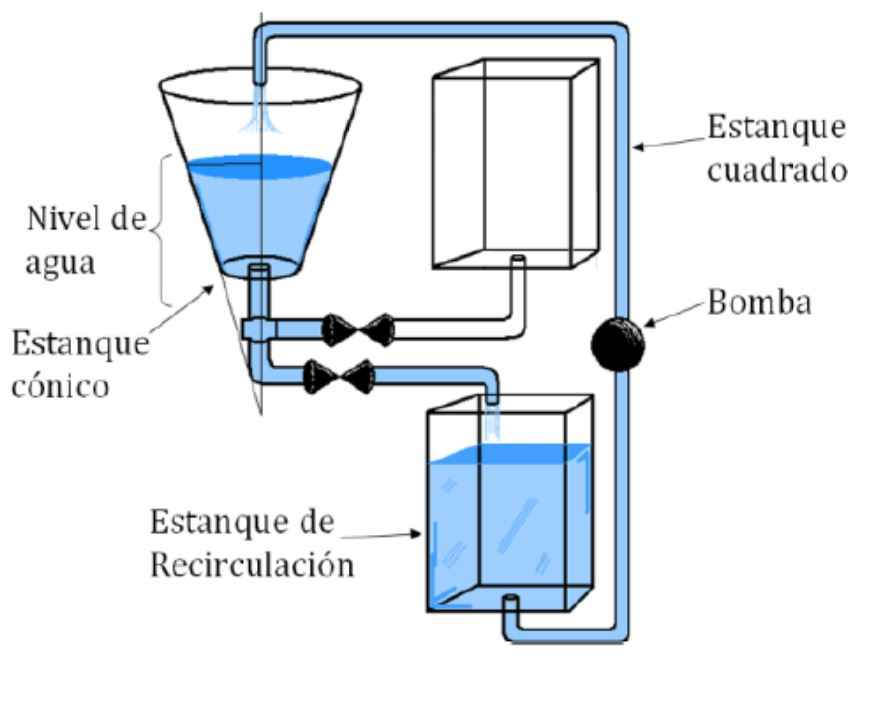
\includegraphics[width=0.5\textwidth]{estanque}
	\caption{Esquema planta.}
	\label{esquema-planta}
\end{center}
\end{figure}

Los estanques cónico y cuadrado poseen una abertura en la parte inferior para que se produzca un flujo de salida de agua por gravitación. Este flujo es captado por cañerías y devuelto al estanque de recirculación, formando un circuito cerrado de flujo de agua, tal como se puede observar en la Figura \ref{flujo}.

\begin{figure}[H]
\begin{center}
	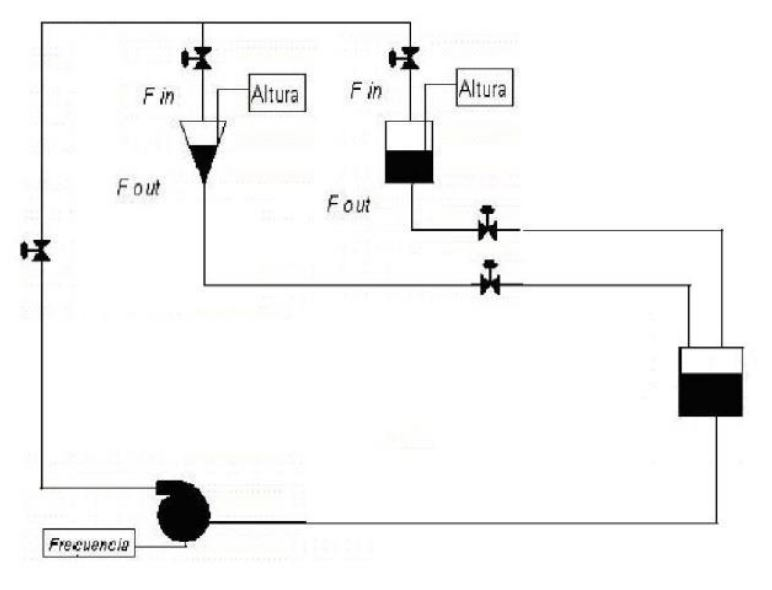
\includegraphics[width=0.5\textwidth]{estanque_flujo}
	\caption{Circuito cerrado de flujo de agua.}
	\label{flujo}
\end{center}
\end{figure}

La función de transferencia que relaciona el flujo impulsado $f_{in}$ (\si{\cubic\centi\metre\per\second}) y el porcentaje de frecuencia de la red $f$ (0-100\%) con que es excitada la bomba, que tiene una velocidad máxima de giro de 2900 (rpm) está dada por:

\begin{equation}
    \frac{f_{in}(s)}{f(s)}=\frac{1.4308}{s+0.15468}
\end{equation}

En este trabajo se diseñarán estrategias de control que permitan controlar el nivel de agua del estanque cuadrado. El nivel de agua (\si{\centi\meter}) es medido mediante un sensor ultrasónico, mientras que el nivel del estanque de recirculación es medido mediante un sensor de presión.

Se desea que el sistema retroalimentado siga las siguientes referencias según sea el caso:

\begin{equation}
\label{ref-r}
r(t) =
  \begin{cases}
    15 \,(\si{\centi\meter})       & \quad 0 \leq t < 200 \,(\si{\second})\\
    20 \,(\si{\centi\meter})       & \quad 200 \leq t < 400 \,(\si{\second})\\
  \end{cases}
\end{equation}

\section{Diseño de controladores para estanque cuadrado}

Para el desarrollo de esta parte considere lo siguiente:

\begin{itemize}

    \item Se cierran las válvulas de entrada y salida del estanque cónico, es decir sólo circulará agua por el estanque cuadrado.
    \item El sensor de medida de nivel de agua en el estanque cuadrado es ideal.
    \item El estanque posee un área basal $A=1681 \,(\si{\square\centi\meter})$.
    \item El flujo de agua entrante depende de la velocidad de giro de la bomba.
    \item Sólo para efectos de modelación considere el flujo de salida cercano a cero, por lo que puede considerarse que es constante e independiente de las diferencias de presión existentes.
    \item La función de transferencia del sistema puede obtenerse a partir de la aplicación de conservación de flujo.
    
\end{itemize}

En esta primera parte del ejercicio se solicita diseñar distintos controladores de nivel para el estanque cuadrado.

\subsection{Actividades}

\begin{enumerate}[\bfseries {A}1]

\item Realice un diagrama de bloques del sistema. Indique cuales son las variables controlada y manipulada, identifique el actuador e indique al menos 2 posibles perturbaciones de la planta.
\item  Plantee las ecuaciones fenomenológicas del sistema utilizando conservación de flujo. Obtenga la función de transferencia del sistema “Estanque cuadrado–bomba”.

\item \label{item-diseno} Mediante lugar geométrico de la raíces diseñe un controlador PI que tenga un tiempo de estabilización de $150\,(\si{\second})$ y una sobre oscilación del 8\%. Estime analíticamente el error en régimen permanente del sistema.

\item Usando MATLAB-Simulink simule la respuesta de lazo cerrado de la planta del usando el controlador diseñado en A\ref{item-diseno} ante la referencia $r(t)$ mostrada en la expresión \ref{ref-r}. Interprete y compare los resultados gráficos.

\end{enumerate}

\section{Control del estanque cuadrado del Laboratorio de Automática}

En esta actividad se implementarán los controladores obtenidos para el estanque cuadrado en en la planta real del el laboratorio.

\subsection{Actividades}
\begin{enumerate}[\bfseries {A}1]
\setcounter{enumi}{4}

\item Realice una prueba del controlador PI discreto utilizando la referencia $r(t)$ con la válvula abierta $45\si{\degree}$ (una marca física muestra este valor).

\item Observe el comportamiento del controlador PI antes diseñado frente a una perturbación en el flujo de salida del sistema utilizando la referencia $r(t)$. Para esto modifique la apertura de la válvula de salida. Comente el desempeño que presentan los controladores luego de realizada esta perturbación. ¿Cómo explicaría las diferencias observadas con el control sin esta perturbación?

\item Abra la válvula de salida completamente. ¿Cómo se comporta controlador ante esta perturbación extrema?

\item Explique y comente en detalle los resultados experimentales obtenidos en los puntos anteriores. Compare los resultados simulados con los obtenidos experimentalmente.

\end{enumerate}



\end{document}